\documentclass[12pt]{article}
\usepackage[left=1.15in, right=1.15in, top=1in, bottom=1.5in]{geometry}
\usepackage{natbib}
\usepackage{verbatim}
\usepackage{setspace}
\usepackage{booktabs}
\usepackage{caption}
\usepackage{graphicx}
\usepackage{subcaption}
\bibpunct[: ]{(}{)}{;}{a}{}{,} 
\usepackage{authblk}
\renewcommand\Authfont{\normalsize}
\renewcommand\Affilfont{\footnotesize}

\begin{document}
\title{Revealing Folk Schemas of Musical Genre and Social Category Associations via Relational and Geometric Methods\thanks{Reserved for acknowledgments}}
\author[1]{Omar Lizardo\thanks{olizardo@soc.ucla.edu}}
\affil[1]{Department of Sociology, UCLA}

\renewcommand\Authands{ and }

\date{\normalsize \today}	
\maketitle

\newpage
\begin{abstract}
\end{abstract}
\newpage
\section*{Introduction}
The notion of musical genre stands as a fundamental concept within the Sociology of Taste, operating as a key organizing principle in understanding cultural consumption and preference \citep{dimaggio1987classification-758, lena2012banding-4b5, lena2008classification-1d7}. Despite its centrality, genre remains a perennially contested category \citep{lena2015relational-21f, vlegels2017music-360}. A core challenge lies in the disparity between intuitive understanding, which suggests that genres are fuzzy, overlapping, and problematic in their boundaries \citep{lizardo2024from-ddd, goldberg2016what-4e3}, and traditional sociological methodologies that often rely on crisp classifications of genre boundaries and measurements of central tendencies \citep{monk2022inequality-699}. This inherent tension has previously led to calls for either outright rejection or radical revision of the genre concept itself \citep{lena2015relational-21f}.

Recent advancements in the field of culture measurement have begun to provide promising avenues for addressing this conundrum. Specifically, relational approaches utilizing network methods and Geometric Data Analysis have emerged, focusing on the inherent fuzziness and overlapping nature of categories \citep{lizardo2024from-ddd}. These methodologies shift the analytical focus towards the distributions of judgments within a relational space \citep{puetz2017fields-f30}. Conceptually, this work employs relational imagery to deconstruct categories as clusters of associations between elements \citep{mcdonnell2024making-b02}, thereby revealing ``folk categories'' by empirically measuring what elements are perceived to ``go with what'' at the level of individual cultural understanding \citep{goldberg2018beyond-f2f}. A key benefit of these approaches is their ability to illuminate heterogeneity across clusters of individuals and cultural items \citep{goldberg2011mapping-77a, vlegels2017music-360}.

Historically, the sociology of taste has concentrated on the objective dual linkage between two primary systems of categories: Genre categories, as developed within cultural production fields like scenes and industries, and social categories, endowed with ritual potency and constitutive of status orders \citep{bourdieu1984distinction-835, bourdieu1993field-8ad, dimaggio1987classification-758, lena2012banding-4b5}. This framework operates on the basic intuition that genres are defined by the types of people who prefer them, and, conversely, categories of people are defined by the genres they choose \citep{breiger2000tool-db3, lizardo2016cultural-aaa}. However, a less common focus in research has been the direct examination of folk construals of these dual linkages, that is, how individuals subjectively perceive the connections between musical genres and social groups \citep{lizardo2016cultural-aaa}.

This paper applies insights derived from the relational, geometric, and schematic turns in measuring culture \citep{goldberg2011mapping-77a, rouanet2000geometric-a44} to the enduring problem of genre within the sociology of taste. My primary objective is to transition analytical perspectives from crisp definitions to fuzzy categories, emphasizing heterogeneity and the distribution of judgments across the social space \citep{romney1986culture-aaa}. Beyond the exclusive focus on objective linkages between genre categories and socio-demographic positions, I aim to investigate folk schemas concerning the subjective folk construals of the link between genre categories and categories of people. By exploiting the sociological duality of genres and social labels \citep{basov2017duality-24b, breiger1974duality-1d0}, I seek to extract detailed associational schemas for both. This involves combining network-analytic and geometric methods to simultaneously examine both central tendencies (centroids) and heterogeneity (variance) in these perceived associations across multiple analytical levels: individual, category, group (demographics), and the broader system.

\section*{Data and Analytic Approach}
To achieve these objectives, I analyze a comprehensive dataset on cultural tastes, collected in the Summer of 2012 from a weighted representative sample of Americans (N = 2,250) \citep{lizardo2016cultural-aaa, lizardo2015musical-8c6, lizardo2024from-ddd}. This dataset, similar to the GSS 1993 survey, includes items assessing respondents' likes, dislikes, and frequency of consumption across twenty distinct musical style categories. Crucially, this dataset incorporates a \textit{perceptual} module that prompted respondents to identify characteristics describing the typical fans of each genre category, allowing them to select all applicable traits from a predefined list of socio-demographic labels (e.g., Male, Female, Young, College Educated, Asian, Black, Hispanic, White, and various social classes). 

\subsection*{Averaged Genre Associations}
Figure~\ref{fig:main} shows a heatmap plot of the proportion of respondents associating each genre with each of the fifteen social labels included in the survey, reproducing one of the key results from \citet[Table 3]{lizardo2016cultural-aaa}. As we can see, respondents use social labels associated with gender fairly indiscriminately, associating them with each genre at a fairly high rate. Racial categories are used in a more discriminating manner, reproducing (on average) standard stereotypes of genre audiences. Rock and traditional ``highbrow" genre categories are associated with white audiences, while Rap, Blues, R\&B, Reggae, and Gospel are associated with Black audiences, and Latin music is associated with Hispanic audiences. The category of Asian is not strongly associated with any genre. Both age and class/education categories also reproduce expected stereotypes. For instance, Rap and Metal are considered ``young'' genres. At the same time, Classic Rock and Country are thought of as ```middle-aged.'' In the same way, Classical and Opera audiences are considered educated and Upper Class, while Bluegrass and Country audiences are considered not college educated and working or lower class. 

\begin{figure}[ht!]
    \centering
    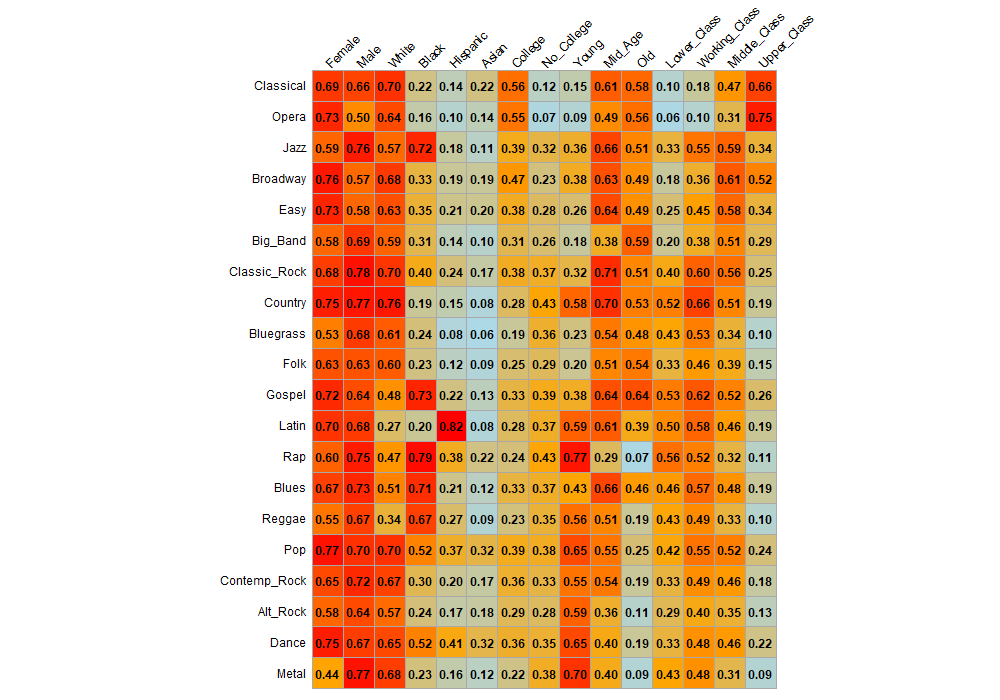
\includegraphics[trim={7cm 0cm 6cm 0cm},clip, width=0.6\textwidth]{Plots/main.png}
    \caption{Heatmap matrix of the proportion of respondents associating each one of fifteen social labels (columns) with one of twenty musical genre categories (rows).}
    \label{fig:main}
\end{figure}

\subsection*{Cognitive Two Mode Networks}
The data used to construct Figure ~\ref{fig:main} consists of averages of more than two thousand binary matrices---one for each respondent---of the same dimensions as~\ref{fig:main} provided by each respondent. As such, the averaging hides as much as it reveals, even as it produces intuitive results. The methodological approach taken here treats this rich disaggregated association data as cognitive two-mode data, conceptually analogous to Krackhardt-style data used in one-mode networks \citep{batchelder1997consensus-f5c, kumbasar1994systematic-213}, where each person provides their perceived associations between musical genres and social labels. In terms of recent work on measuring culture, each person-level two-mode data table records the (explicit) schematic structure of how individuals perceive each genre category relative to the set of social labels \citep{hunzaker2019mapping-280}.

More formally, each individual provides a ``personal'' two mode network of genres by social labels with corresponding affiliation matrix $\mathbf{A}(p)$, where $a^{(p)}_{gl} = 1$ if individual $p$ associates genre $g$ with label $l$. Following \citet{breiger1974duality-1d0}, the personal genre projection is given by:

\begin{equation}
   \mathbf{G}(p) = \mathbf{A}(p)\mathbf{A}(p)^T 
\end{equation}

Where $g^{(p)}_{ij}$ records the $p^{th}$ individual's perceived similarity between genres $i$ and $j$ based on their shared labels and $g^{(p)}_{ii}$ records the number of times individual $p$ associates genre $i$ with a label.

In the same way, the personal label projection is given by:

\begin{equation}
    \mathbf{L}(p) = \mathbf{A}(p)^T\mathbf{A}(p)
\end{equation}
 
Where $l^{(p)}_{kl}$ records the $p^{th}$ individual's perceived similarity between labels $k$ and $l$ based on their shared genres, and $l^{(p)}_{kk}$ records the number of times individual $p$ associates genre $i$ with a label. The structure of the data thus allows us to take a ``Mondo Breiger'' approach \citep{lee2018doorway-008}, where we can perform dual projections at the level of each individual. 

\subsection*{Individual Backbone Extraction}
Because each dual projection is likely to over-estimate the perceived similarities between genres and labels at the level of the individual, I use backbone extraction on each individual-level projection---more specifically, the Stochastic Degree Sequence Model (SDSM)---to isolate the most significant genre-to-genre and label-to-label associations for each person \citep{neal2014backbone-b29}. 

The SDSM works as follows: In the first step, a generalized linear model for binary outcomes is used to predict the probability of a tie between each genre and label in the two-mode network, using the number of times a genre was associated with social label and the number of times a social label was associated with a genre (the degrees of the nodes in each mode) and their interaction as predictors. From the predicted probabilities derived from this model (where the unit of analysis is the genre/label pair), we create an ensemble of two-mode networks, generate genre-to-genre and label-to-label projections for each, and compute the proportion of times that the projected edge weight between pairs of genres and pairs of labels is smaller in the generated projection ensemble than that observed in the original network projection. We then assign a binary link between two genres and two labels in the corresponding backbone (indicating perceived similarity) if this percentage falls below a certain threshold. In these data, the usual $p < 0.05$ criterion proves to be too strong (generating mostly empty backbones) for each genre-to-genre and label-to-label projection. Accordingly, I use a less stringent criterion of $p < 0.45$.  

\begin{figure}[ht!]
    \captionsetup[subfigure]{font=footnotesize,labelfont=footnotesize}
    \centering
     \begin{subfigure}[b]{0.49\textwidth}
        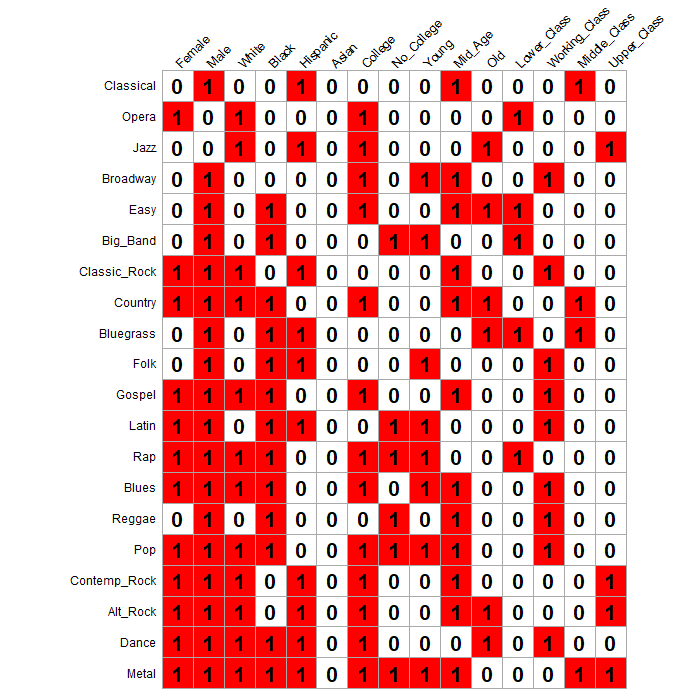
\includegraphics[trim={4cm 0cm 3cm 0cm},clip, width=0.9\textwidth]{Plots/data-ex-af1.png}
            \caption{Case ID: 65}
            \label{fig:ind-ex-aff1}
    \end{subfigure}
     \begin{subfigure}[b]{0.49\textwidth}
        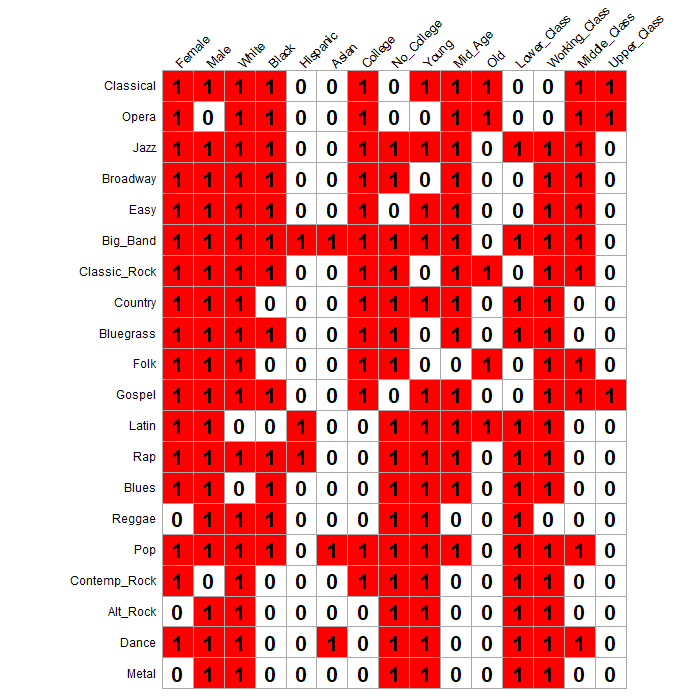
\includegraphics[trim={4cm 0cm 3cm 0cm},clip, width=0.9\textwidth]{Plots/data-ex-af2.png}
            \caption{Case ID: 236}
            \label{fig:ind-ex-aff2}
    \end{subfigure}
    \caption{Individual affiliation matrices of the association between musical genres and social labels.}
    \label{fig:ind-ex-aff}
\end{figure}

Figure~\ref{fig:ind-ex-aff} shows the cognitive two-mode network matrices of the associations between genres and social labels for two individuals in the data. It is clear from this example that the averaged associations shown in Figure~\ref{fig:main} hide quite a lot of individual variation and idiosyncratic perceptions. For instance, Case ID 65 believes that Heavy Metal encompasses most types of people, regardless of gender and race (excluding Asians), but thinks that Jazz music only appeals to older white or Hispanic people with a college degree. Case ID 236, on the other hand, thinks that Metal fans are mostly young white men without a college degree, but the classical appeals to most people regardless of gender, race, and age.  

\begin{figure}[ht!]
    \captionsetup[subfigure]{font=footnotesize,labelfont=footnotesize}
    \centering
     \begin{subfigure}[b]{0.49\textwidth}
        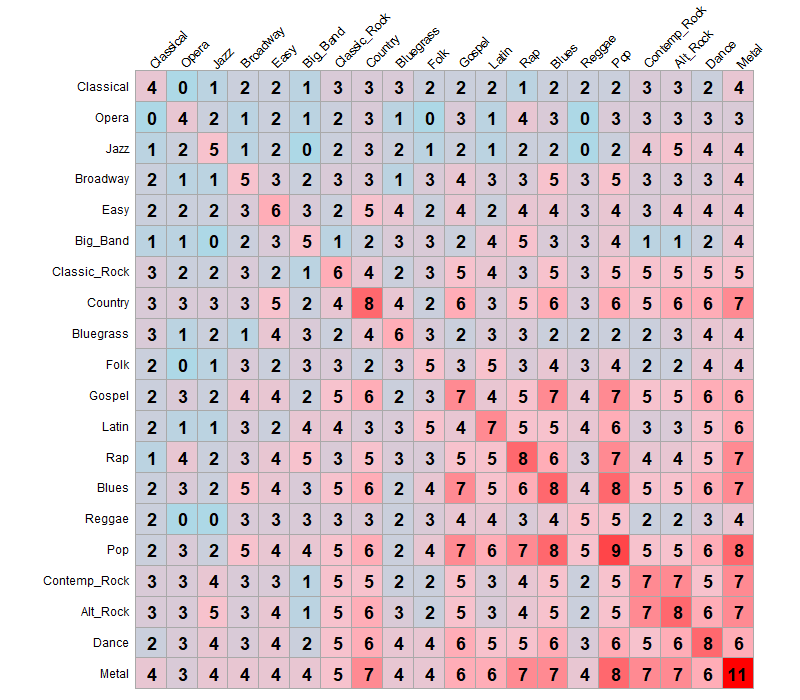
\includegraphics[trim={1cm 0cm 0cm 0cm},clip, width=0.9\textwidth]{Plots/data-ex-rp1.png}
            \caption{Case ID: 65}
            \label{fig:ind-ex-rp1}
    \end{subfigure}
     \begin{subfigure}[b]{0.49\textwidth}
        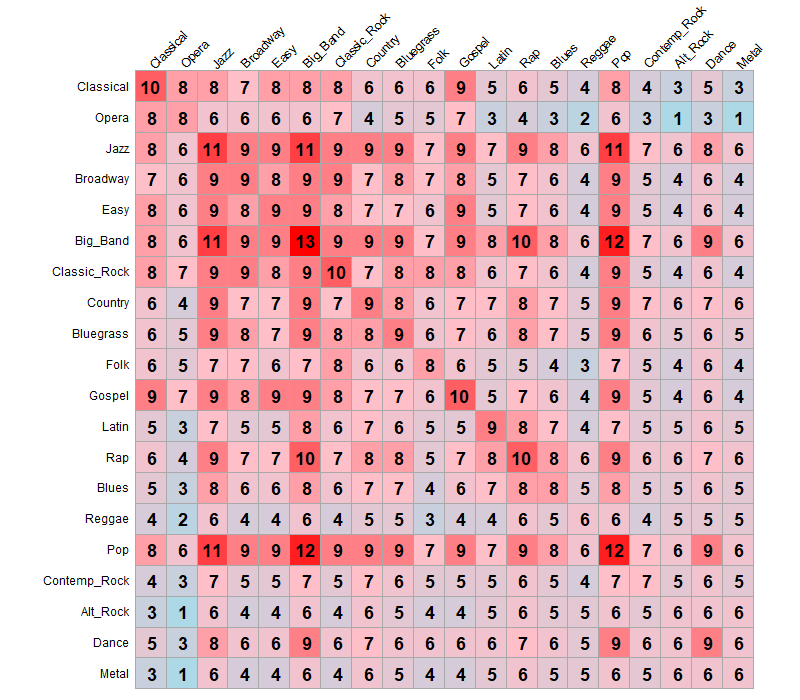
\includegraphics[trim={1cm 0cm 0cm 0cm},clip, width=0.9\textwidth]{Plots/data-ex-rp2.png}
            \caption{Case ID: 236}
            \label{fig:ind-ex-rp2}
    \end{subfigure}
     \begin{subfigure}[b]{0.49\textwidth}
        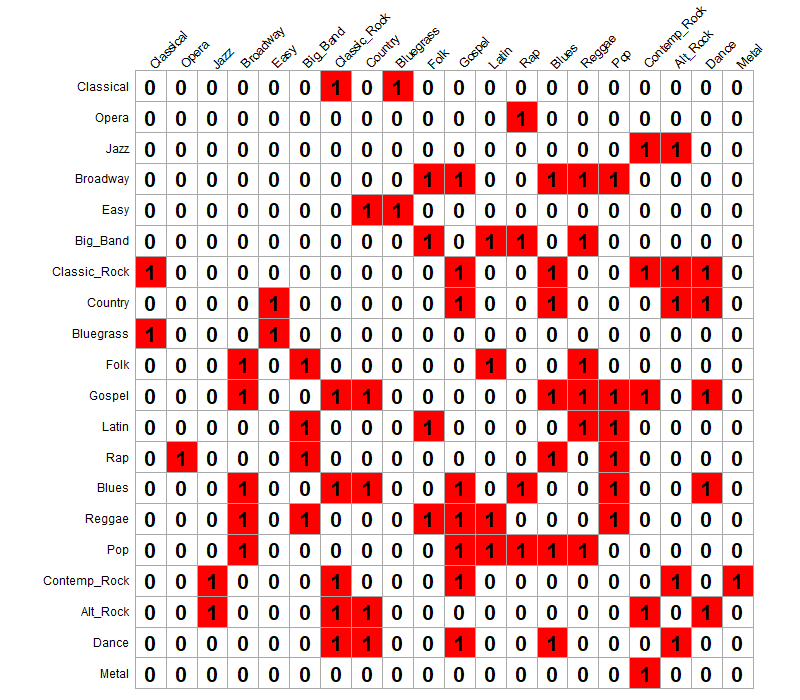
\includegraphics[trim={1cm 0cm 0cm 0cm},clip, width=0.9\textwidth]{Plots/data-ex-rbb1.png}
            \caption{Case ID: 65}
            \label{fig:ind-ex-rbb1}
    \end{subfigure}
     \begin{subfigure}[b]{0.49\textwidth}
        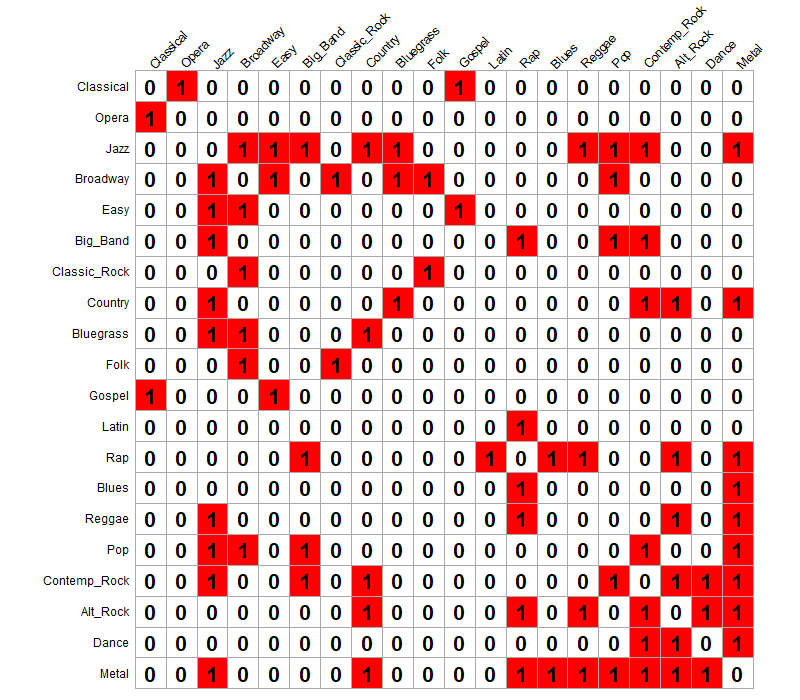
\includegraphics[trim={1cm 0cm 0cm 0cm},clip, width=0.9\textwidth]{Plots/data-ex-rbb2.png}
            \caption{Case ID: 236}
            \label{fig:ind-ex-rbb2}
    \end{subfigure}
    \caption{Individual genre backbones.}
    \caption{Individual genre projection matrices and corresponding backbones.}
    \label{fig:ind-ex-rp}
\end{figure}

Figure~\ref{fig:ind-ex-rp} shows the individual row projections ($\mathbf{G}(p)$) and corresponding backbones for each of these two cases, encoding the perceived similarities between genres and social labels for each individual. We can see, for instance, that in accordance with their cognitive two-mode network, which sees the Metal audience as relatively undifferentiated, Case ID 65 does not strongly associate Metal with any other genre, except contemporary rock. In the same way, Case ID 236 sees Classical and Opera as strongly linked, and Metal as most similar to such genres as Reggae, Rap, Alt Rock, and Contemporary Rock. The corresponding column projections ($\mathbf{L}(p)$) and backbones for these two cases are shown in Figure~\ref{fig:ind-ex-cp}. Both individuals associate white people with a college degree; Case ID 65 sees the label ``Working Class'' as most similar to ``Black'' and ``Young,'' but Case ID 263 sees the same label as most similar to ``Hispanic," ``Asian,'' and people without a college education. 

\begin{figure}[ht!]
    \captionsetup[subfigure]{font=footnotesize,labelfont=footnotesize}
    \centering
     \begin{subfigure}[b]{0.49\textwidth}
        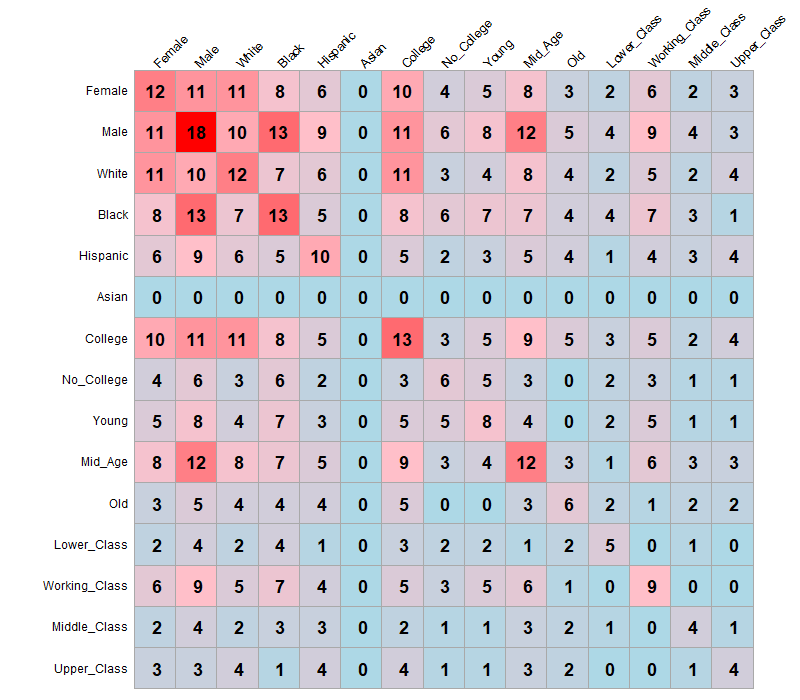
\includegraphics[trim={1cm 0cm 0cm 0cm},clip, width=0.9\textwidth]{Plots/data-ex-cp1.png}
            \caption{Case ID: 65}
            \label{fig:ind-ex-cp1}
    \end{subfigure}
     \begin{subfigure}[b]{0.49\textwidth}
        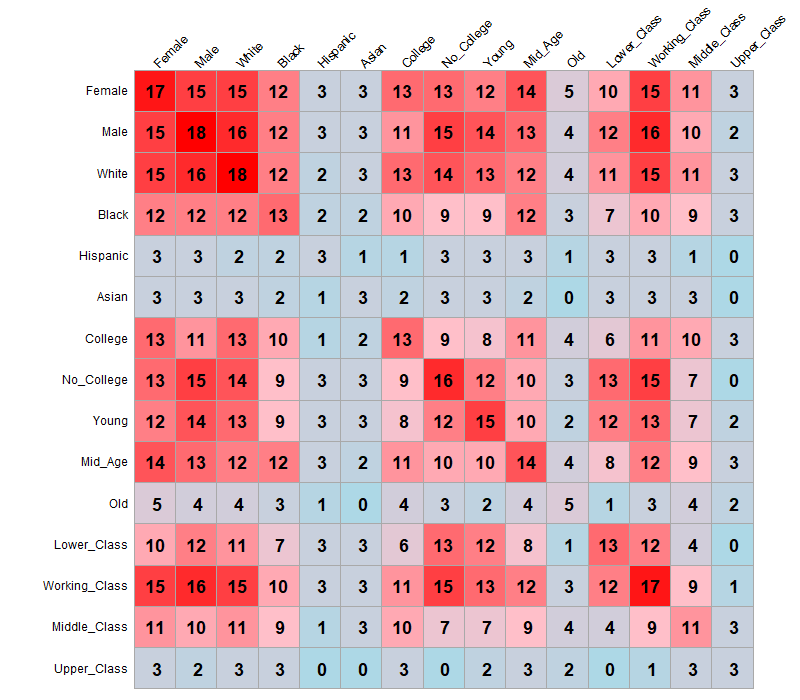
\includegraphics[trim={1cm 0cm 0cm 0cm},clip, width=0.9\textwidth]{Plots/data-ex-cp2.png}
            \caption{Case ID: 236}
            \label{fig:ind-ex-cp2}
    \end{subfigure}
     \begin{subfigure}[b]{0.49\textwidth}
        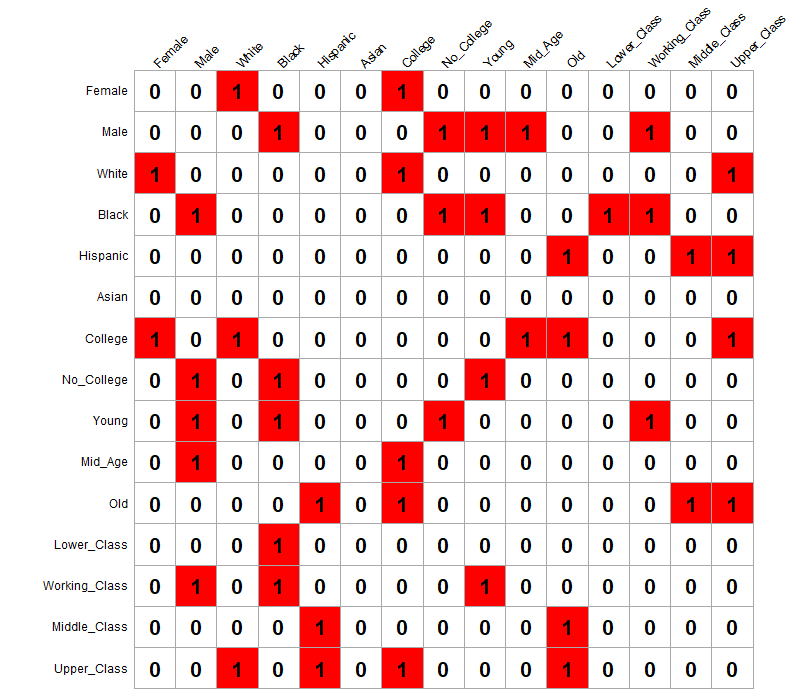
\includegraphics[trim={1cm 0cm 0cm 0cm},clip, width=0.9\textwidth]{Plots/data-ex-cbb1.png}
            \caption{Case ID: 65}
            \label{fig:ind-ex-cbb1}
    \end{subfigure}
     \begin{subfigure}[b]{0.49\textwidth}
        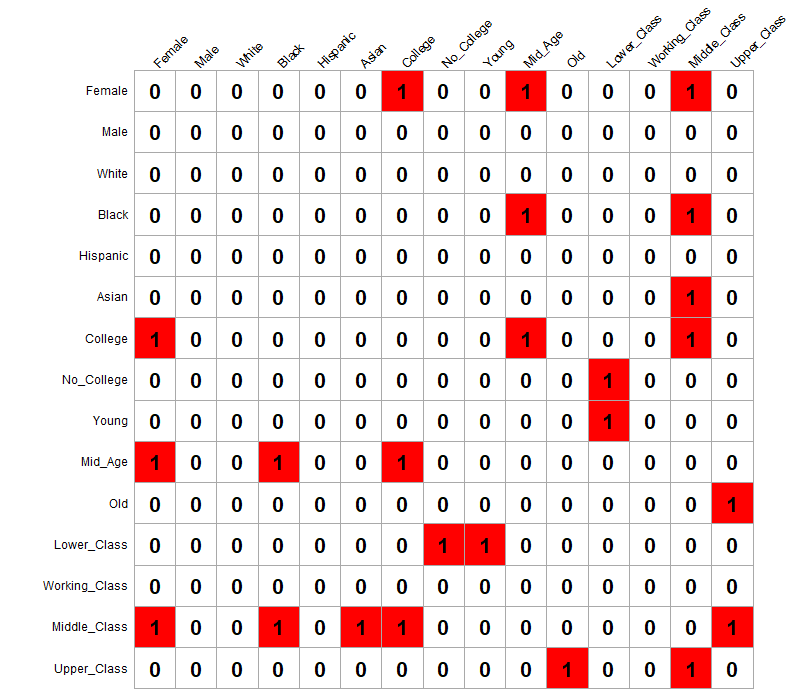
\includegraphics[trim={1cm 0cm 0cm 0cm},clip, width=0.9\textwidth]{Plots/data-ex-cbb2.png}
            \caption{Case ID: 236}
            \label{fig:ind-ex-cbb2}
    \end{subfigure}
    \caption{Individual label projection matrices and corresponding backbones.}
    \label{fig:ind-ex-cp}
\end{figure}

\section*{Workflow Illustration}
Once we have computed the genre and label projection backbones for each individual in the survey, we stack these matrices, generating two tables of dimensions $(N \times 20) \times 20$ (for genres) and $(N \times 15) \times 20$ (for labels). We applied the subject of each of these to Correspondence Analysis (CA) to obtain consensus (column) scores of the similarity between genres and labels, along with individual perceptions of the placement of each genre and label in the same spaces (row scores) \citep{kumbasar1994systematic-213}. These scores are then analyzed using Geometric Data Analytic methods \citep{rouanet2000geometric-a44}.

\begin{figure}[ht!]
    \captionsetup[subfigure]{font=footnotesize,labelfont=footnotesize}
    \centering
        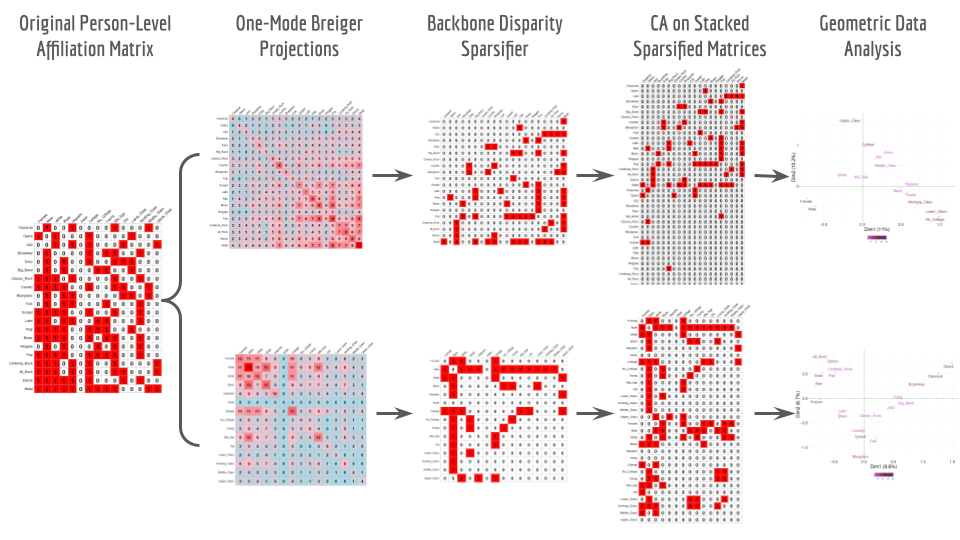
\includegraphics[trim={1cm 0cm 0cm 0cm},clip, width=0.9\textwidth]{mondo-workflow.png}
    \caption{Individual label projection matrices and corresponding backbones.}
    \label{fig:ind-ex-cp}
\end{figure}


This analytical framework thus generates three sets of scores: person-specific judgments of the relative similarity of genres and labels (row scores), aggregate judgments of genre and label similarity (column scores), and supplementary scores for genres and labels representing the centroid of the cloud of person-specific judgments. Ultimately, this allows me to examine heterogeneity in folk understandings by observing how multiple clouds of individuals (projected into both genre and social label spaces) distribute themselves along principal axes, providing critical insights into the variation in meaning consensus across different levels of analysis. The resulting data workflow is shown in Figure


\section*{Results}

\section*{Discussion and Conclusions}

\newpage
\bibliography{references}
\bibliographystyle{apalike}
\end{document}